This chapter briefly describes how to insert figures and tables (especially those that are rotated 90 degrees, which are very common in theses).

\section{Figure}
When you want to create a TikZ figure, you can use the online tool \texttt{Mathcha.io}\footnote{\url{https://www.mathcha.io/editor}}.


\begin{figure}
\centering
\tikzset{every picture/.style={line width=0.75pt}} %set default line width to 0.75pt
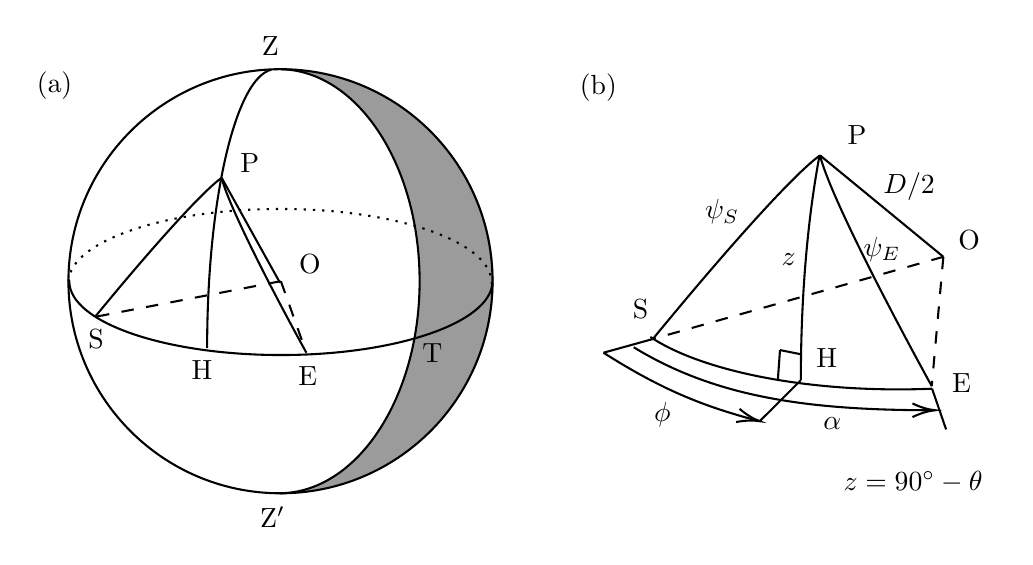
\begin{tikzpicture}[x=0.75pt,y=0.75pt,yscale=-1,xscale=1]

%uncomment if require:\path (0,476.33333587646484); %set diagram left start at 0, and has height of 476.33333587646484

%Shape:Arc [id:dp9200567780243829]
\draw  [draw opacity=0][fill={rgb, 255:red, 155; green, 155; blue, 155 }  ,fill opacity=1 ] (189.77,24) .. controls (246.05,24.43) and (291.54,70) .. (291.54,126.16) .. controls (291.54,182.44) and (245.87,228.08) .. (189.43,228.33) -- (188.96,126.16) -- cycle ; \draw  [draw opacity=0] (189.77,24) .. controls (246.05,24.43) and (291.54,70) .. (291.54,126.16) .. controls (291.54,182.44) and (245.87,228.08) .. (189.43,228.33) ;
%Shape:Arc [id:dp7489325740381287]
\draw  [draw opacity=0][fill={rgb, 255:red, 255; green, 255; blue, 255 }  ,fill opacity=1 ] (188.83,24) .. controls (225.93,24.65) and (255.87,70.14) .. (255.87,126.16) .. controls (255.87,182.36) and (225.75,227.96) .. (188.49,228.33) -- (188.03,126.16) -- cycle ; \draw   (188.83,24) .. controls (225.93,24.65) and (255.87,70.14) .. (255.87,126.16) .. controls (255.87,182.36) and (225.75,227.96) .. (188.49,228.33) ;
%Shape:Circle [id:dp03629587840911208]
\draw   (86.67,126.17) .. controls (86.67,69.74) and (132.41,24) .. (188.83,24) .. controls (245.26,24) and (291,69.74) .. (291,126.17) .. controls (291,182.59) and (245.26,228.33) .. (188.83,228.33) .. controls (132.41,228.33) and (86.67,182.59) .. (86.67,126.17) -- cycle ;
%Shape:Arc [id:dp7942338684517938]
\draw  [draw opacity=0] (290.97,126.89) .. controls (289.85,146.19) and (244.64,161.72) .. (189.04,161.72) .. controls (132.73,161.72) and (87.08,145.8) .. (87.08,126.16) .. controls (87.08,126.02) and (87.09,125.88) .. (87.09,125.74) -- (189.04,126.16) -- cycle ; \draw   (290.97,126.89) .. controls (289.85,146.19) and (244.64,161.72) .. (189.04,161.72) .. controls (132.73,161.72) and (87.08,145.8) .. (87.08,126.16) .. controls (87.08,126.02) and (87.09,125.88) .. (87.09,125.74) ;
%Shape:Arc [id:dp9629399739735423]
\draw  [draw opacity=0][dash pattern={on 0.84pt off 2.51pt}] (86.67,126.17) .. controls (87.78,106.87) and (132.99,91.34) .. (188.6,91.34) .. controls (244.9,91.34) and (290.55,107.26) .. (290.55,126.9) .. controls (290.55,127.04) and (290.55,127.18) .. (290.54,127.32) -- (188.6,126.9) -- cycle ; \draw  [dash pattern={on 0.84pt off 2.51pt}] (86.67,126.17) .. controls (87.78,106.87) and (132.99,91.34) .. (188.6,91.34) .. controls (244.9,91.34) and (290.55,107.26) .. (290.55,126.9) .. controls (290.55,127.04) and (290.55,127.18) .. (290.54,127.32) ;
%Straight Lines [id:da7427330116367932]
\draw    (188.6,126.9) -- (160.5,76.33) ;


%Shape:Arc [id:dp3533944543316787]
\draw  [draw opacity=0] (153.5,158.35) .. controls (153.5,158.29) and (153.5,158.23) .. (153.5,158.16) .. controls (153.5,86.72) and (167.2,28.32) .. (184.48,24.22) -- (186.42,158.16) -- cycle ; \draw   (153.5,158.35) .. controls (153.5,158.29) and (153.5,158.23) .. (153.5,158.16) .. controls (153.5,86.72) and (167.2,28.32) .. (184.48,24.22) ;
%Shape:Arc [id:dp24905583167207346]
\draw  [draw opacity=0] (201.26,160.52) .. controls (178.79,119.6) and (162.99,87.01) .. (160.5,76.33) -- (227.42,189.04) -- cycle ; \draw   (201.26,160.52) .. controls (178.79,119.6) and (162.99,87.01) .. (160.5,76.33) ;
%Shape:Arc [id:dp6265901038149739]
\draw  [draw opacity=0] (99.49,143.34) .. controls (128.21,108.36) and (151.72,82.5) .. (160.5,76.33) -- (80.96,180.52) -- cycle ; \draw   (99.49,143.34) .. controls (128.21,108.36) and (151.72,82.5) .. (160.5,76.33) ;
%Straight Lines [id:da7398895483577017]
\draw  [dash pattern={on 4.5pt off 4.5pt}]  (188.83,126.17) -- (99.49,143.34) ;


%Straight Lines [id:da705866788910704]
\draw  [dash pattern={on 4.5pt off 4.5pt}]  (189.04,126.16) -- (201.26,160.52) ;


%Shape:Arc [id:dp37174002489256974]
\draw  [draw opacity=0] (502.78,177.94) .. controls (497.43,178.16) and (491.99,178.28) .. (486.47,178.28) .. controls (434.55,178.28) and (389.49,168.03) .. (367.04,153.01) -- (486.47,131.33) -- cycle ; \draw   (502.78,177.94) .. controls (497.43,178.16) and (491.99,178.28) .. (486.47,178.28) .. controls (434.55,178.28) and (389.49,168.03) .. (367.04,153.01) ;
%Straight Lines [id:da037701469103981866]
\draw    (508.21,114.39) -- (448.79,65.53) ;


%Shape:Arc [id:dp5716767409377437]
\draw  [draw opacity=0] (439.55,173.83) .. controls (439.55,173.75) and (439.55,173.66) .. (439.55,173.58) .. controls (439.55,132.9) and (442.91,95.42) .. (448.57,65.52) -- (483.01,173.58) -- cycle ; \draw   (439.55,173.83) .. controls (439.55,173.75) and (439.55,173.66) .. (439.55,173.58) .. controls (439.55,132.9) and (442.91,95.42) .. (448.57,65.52) ;
%Shape:Arc [id:dp9649704010073819]
\draw  [draw opacity=0] (502.61,176.7) .. controls (472.95,122.66) and (452.08,79.63) .. (448.79,65.53) -- (537.15,214.35) -- cycle ; \draw   (502.61,176.7) .. controls (472.95,122.66) and (452.08,79.63) .. (448.79,65.53) ;
%Shape:Arc [id:dp8065254293203821]
\draw  [draw opacity=0] (368.23,154.01) .. controls (406.16,107.82) and (437.19,73.68) .. (448.79,65.53) -- (343.76,203.1) -- cycle ; \draw   (368.23,154.01) .. controls (406.16,107.82) and (437.19,73.68) .. (448.79,65.53) ;
%Straight Lines [id:da8597935314379497]
\draw  [dash pattern={on 4.5pt off 4.5pt}]  (508.21,114.39) -- (368.23,154.01) ;


%Straight Lines [id:da7419733626645719]
\draw  [dash pattern={on 4.5pt off 4.5pt}]  (508.21,114.39) -- (502.61,176.7) ;


%Straight Lines [id:da7639447353983435]
\draw    (368.23,154.01) -- (344.48,160.6) ;


%Straight Lines [id:da20604704739410318]
\draw    (439.55,173.83) -- (419.74,193.61) ;


%Straight Lines [id:da3289024362291044]
\draw    (502.78,177.94) -- (509.53,197.57) ;


%Curve Lines [id:da4960441686676247]
\draw    (344.48,160.6) .. controls (373.44,179.06) and (393.62,186.63) .. (417.87,193.12) ;
\draw [shift={(419.74,193.61)}, rotate = 194.74] [color={rgb, 255:red, 0; green, 0; blue, 0 }  ][line width=0.75]    (10.93,-3.29) .. controls (6.95,-1.4) and (3.31,-0.3) .. (0,0) .. controls (3.31,0.3) and (6.95,1.4) .. (10.93,3.29)   ;

%Curve Lines [id:da5236116047062247]
\draw    (359,157.96) .. controls (399.52,182.8) and (445.22,188.22) .. (502.51,188.33) ;
\draw [shift={(504.25,188.33)}, rotate = 180] [color={rgb, 255:red, 0; green, 0; blue, 0 }  ][line width=0.75]    (10.93,-3.29) .. controls (6.95,-1.4) and (3.31,-0.3) .. (0,0) .. controls (3.31,0.3) and (6.95,1.4) .. (10.93,3.29)   ;

%Straight Lines [id:da6896999351783069]
\draw    (439.5,161.33) -- (429.5,159.33) ;


%Straight Lines [id:da5299534706716347]
\draw    (428.5,173.33) -- (429.5,159.33) ;



% Text Node
\draw (174,69) node   {$\mathrm{P}$};
% Text Node
\draw (184,13) node   {$\mathrm{Z}$};
% Text Node
\draw (100,154) node   {$\mathrm{S}$};
% Text Node
\draw (202,172) node   {$\mathrm{E}$};
% Text Node
\draw (151,169) node   {$\mathrm{H}$};
% Text Node
\draw (203,118) node   {$\mathrm{O}$};
% Text Node
\draw (185,240) node   {$\mathrm{Z}^{\prime }$};
% Text Node
\draw (262,161) node   {$\mathrm{T}$};
% Text Node
\draw (466.61,55.85) node   {$\mathrm{P}$};
% Text Node
\draw (362.38,139.68) node   {$\mathrm{S}$};
% Text Node
\draw (517.03,175.41) node   {$\mathrm{E}$};
% Text Node
\draw (452.04,163.3) node   {$\mathrm{H}$};
% Text Node
\draw (520.6,106.35) node   {$\mathrm{O}$};
% Text Node
\draw (372.87,190.53) node   {$\phi $};
% Text Node
\draw (454.73,194.49) node   {$\alpha $};
% Text Node
\draw (401.67,92.82) node   {$\psi _{S}$};
% Text Node
\draw (478.66,110.79) node   {$\psi _{E}$};
% Text Node
\draw (433.67,115.82) node   {$z$};
% Text Node
\draw (80,32) node  [align=left] {(a)};
% Text Node
\draw (342,33) node  [align=left] {(b)};
% Text Node
\draw (493.67,222.82) node   {$z=90^{\circ } -\theta $};
% Text Node
\draw (491.66,80.79) node   {$D/2$};
\end{tikzpicture}
\caption[A schematic diagram (This is the title appear in ``List of Figures'')]{The schematic diagram for the NEATM formalism. (a) blah blah blah blah blah blah blah blah blah blah blah blah blah blah blah blah. (b) blah blah blah blah blah blah blah blah blah blah blah blah blah blah blah blah blah blah blah blah blah blah blah blah blah blah blah blah blah blah blah blah. Figure from Bach Y. P. PhD thesis (2023)}
\label{fig:schematic}
\end{figure}


\section{Table}
A frequent usage is to use \texttt{tabular} inside \texttt{table}, as in \Cref{tab: gR value}.


\begin{table*}[!tb]
\centering
  \caption[The parameter values.]{Brief explanation, blah blah blah blah blah blah blah blah blah blah blah blah blah blah blah blah. Table from \cite{2022_SAG_NICpolpy}.}
  \label{tab: gR value}
    \begin{tabular}{cc|ccc|c}
      \hline\hline
       & & \multicolumn{2}{c}{\citet{Ishiguro2011ARNHAO}} & This work & Adopted value \\
      Parameter & Detector  & Motor ON & Motor OFF & ($\mathrm{mean} \pm \mathrm{std} $) & in \texttt{NICpolpy}\\
      \hline
                   &J-band & $ 4.7 \pm 0.5 $ & $ 5.4 \pm 0.5 $ &                     & \\
      $ R/g $ [ADU]&H-band & $ 8.8 \pm 0.6 $ & $ 7.7 \pm 0.4 $ &  $ 3.7 (\pm <0.1) $ & $ (3.7) $\\
                   &K-band & N/A             & $ 8.8 \pm 0.6 $ &                     & \\
      \hline
                   &J-band & $ 9.8 \pm 0.2 $ & $ 9.2 \pm 0.2 $ & $ 9.9 \pm 1.0 $ & $ 9.9 $\\
      $ g $ [e/ADU]&H-band & $ 9.5 \pm 0.2 $ & $ 9.8 \pm 0.2 $ & $ 9.8 \pm 0.9 $ & $ 9.8 $\\
                   &K-band & N/A             & $ 9.4 \pm 0.2 $ & $ 9.5 \pm 0.9 $ & $ 9.5 $\\
      \hline
                   &J-band & $ 46 \pm 5 $ & $ 50 \pm 4 $ & $ 37 \pm 4 $ & $ 37 $ \\
      $ R $ [e]    &H-band & $ 84 \pm 5 $ & $ 75 \pm 4 $ & $ 36 \pm 3 $ & $ 36 $ \\
                   &K-band & $ (>250) $   & $ 83 \pm 5 $ & $ 35 \pm 3 $ & $ 35 $ \\
      \hline
    \end{tabular}
\end{table*}




\section{Large Figure/Table}
If the figure is large, you can rotate it using \texttt{$\backslash$begin\{sidewaysfigure\}[!ph]} as in \Cref{fig:flatinsrot}. Similarly, if the table is large, you can use \texttt{$\backslash$begin\{sidewaystable\}[!ph]} as in \Cref{tab: notation}.


\begin{sidewaysfigure} [!ph]
  \begin{center}
    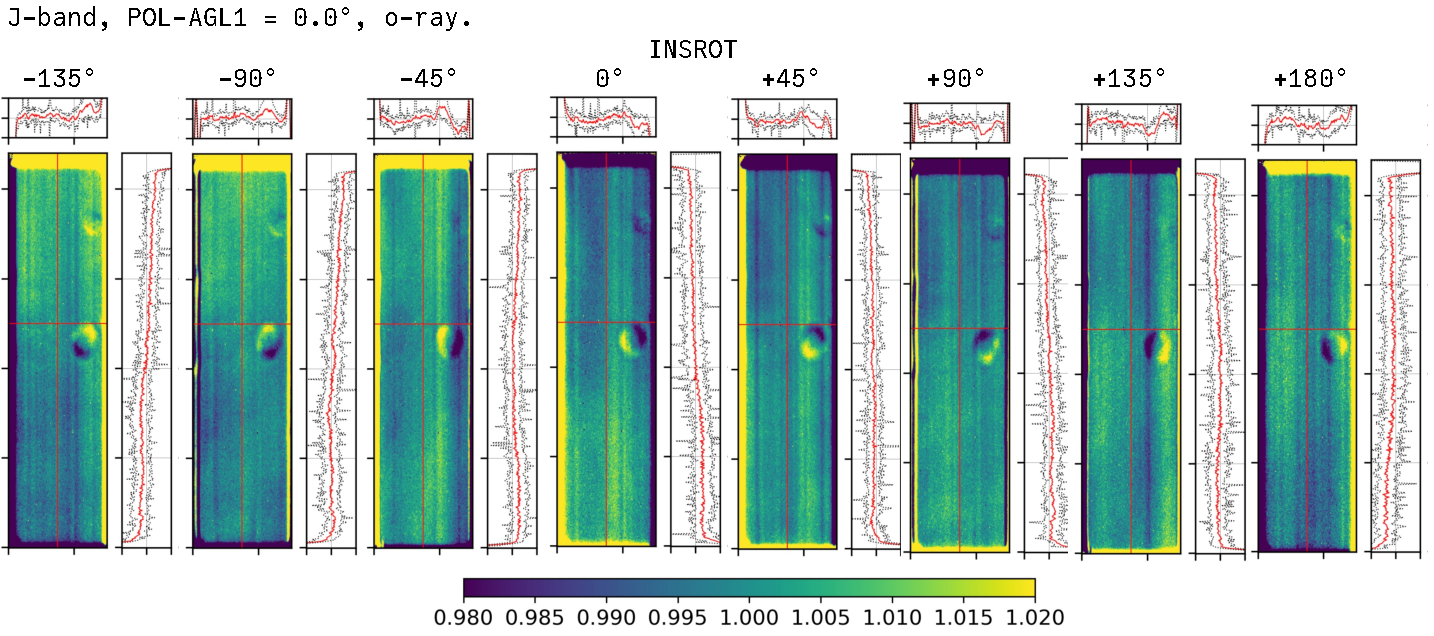
\includegraphics[width=\linewidth]{figs/flatinsrot.pdf}
  \end{center}
  \caption[The $ r_1 $ ratio map for J-band with HWP rotator angle $ 0^\circ $ and o-ray region only.]{Explanation, blah blah blah blah blah blah blah blah blah blah blah blah blah blah blah blah. Figure from \cite{2022_SAG_NICpolpy}.}
  \label{fig:flatinsrot}
\end{sidewaysfigure}



\begin{sidewaystable}[!ph]
  \centering
  \caption[Symbols frequently used in this paper.]{Explanation blah blah blah blah blah blah blah blah blah blah blah blah blah blah blah blah Table is from \cite{2019JKAS...52...71B}.}
  \label{tab: notation}
  \setlength{\tabcolsep}{19pt}
  \begin{tabular}{llll}
    \hline\hline
    Category & Symbols & Description & Value and Unit \\  % Table Heading
    \hline
    Magnitudes
     & $ V_\odot $         & Visual magnitude of the Sun           & $ -26.762 \mathrm{(mag)} $       \\
     & $ V $, $ \Delta V $ & Visual magnitude and its uncertainty  & $ \mathrm{(mag)} $ \\
     & $ \HVa $            & Reduced magnitude                     & $ \mathrm{(mag)} $ \\
     & $ \HV $             & Absolute magnitude ($ \coloneqq \HV(0) $) & $ \mathrm{(mag)} $ \\
     & $ G $               & Slope parameter                       & ~~ --- \\
    \hline
    Ephemerides
     & $ \rhel $, $ \robs $           & Heliocentric/geocentric distance          & $ \mathrm{m} $ or $ \mathrm{au} $ \\
     & $ \alpha $                 & Phase angle                               & ($ \mathrm{\degr} $ or $ \mathrm{rad} $) \\
     & $ t $                      & Time on the target (light-time corrected) & $ \mathrm{s} $ or $ \mathrm{JD} $ \\
     & $ (\lambda,\, \beta) $     & Ecliptic coordinate (longitude, latitude) & ($ \mathrm{\degr} $ or $ \mathrm{rad} $) \\
%     & $ (\lambda_\h,\, \beta_\h)_\mathrm{h.e.} $
%                                  & Heliocentric $ (\lambda, \beta) $         & ($ \mathrm{\degr} $ or $ \mathrm{rad} $) \\
%     & $ (\lambda_\g,\, \beta_\g)_\mathrm{g.e.} $
%                                  & Geocentric $ (\lambda, \beta) $           & ($ \mathrm{\degr} $ or $ \mathrm{rad} $) \\
%    \hline
%    Rotation
%     & $ \spin_1 $, $ \spin_2 $
%                                & Rotational/precessional vector              & ($ \mathrm{\degr} $, $ \mathrm{\degr} $)  \\
%     & $ P_1 $, $ P_2 $           & Rotational/precessional period            & $ \mathrm{s} $ or $ \mathrm{day} $ \\
%     & $ \omega_1 $, $ \omega_2 $ & Rotational/precessional angular speed     & $ \mathrm{s^{-1}} $ ($ \mathrm{rad/s} $) \\
%     & $ \varphi_1 $, $ \varphi_2 $ & Rotational/precessional phase offset    & ($ \mathrm{rad} $) \\
    \hline
    Physical
     & $ S_\mathrm{proj} $      & Total projected area viewed at $ \alpha = 0 $ & $ \mathrm{m^2} $ \\
    parameters
     & $ D $           & Effective diameter                                   & $ \mathrm{m} $ or $ \km $\\
     & $ \pV $         & Geometric albedo in visual (V) band                  & ~~ --- \\
     & $ A_5 $         & Albedo at the phase angle of $ \alpha = 5 \degr $    & ~~ --- \\
     & $ I $           & The irradiance of the object of interest             & $ \mathrm{W/m^2} $ \\
     & $ F $           & $ I $ of a Lambertian reflector at normal incidence  & $ \mathrm{W/m^2} $ \\
     & $ I/F $         & The radiance factor                                  & ~~ --- \\
    \hline
  \end{tabular}
\end{sidewaystable}

